\documentclass[tikz,border=50mm]{standalone}
% !TeX program = luatex

%===This is the preambule I call in every file===

\usepackage{tikz}
\usepackage{xcolor}
\usepackage{pgfplots}
\usepackage{circuitikz}
\usepackage{tikz-3dplot}
\pgfplotsset{compat=newest}
\usetikzlibrary{arrows.meta, shapes.geometric, positioning, perspective, patterns.meta, decorations.pathreplacing, decorations.pathmorphing, decorations.markings, patterns, arrows.meta, shapes, shapes.geometric, decorations.text, angles, quotes,calc, 3d, math, circuits.ee.IEC,hobby, knots, intersections, through}


%=== The Euler Med Logo ===
%=== i.e. My signature ===

\usepackage{amsmath, amsfonts}
\makeatletter
\newcommand*\eulermed{{
\scalebox{3.3}{$\mathbb{E}$}\kern-1pt \scalebox{1.5}{u$\ell\varepsilon\rho$}\kern-55pt
\raisebox{19pt}{\scalebox{1.5}{$\mathcal{M}\varepsilon\delta$}}}
\@}
\makeatother

\begin{document}
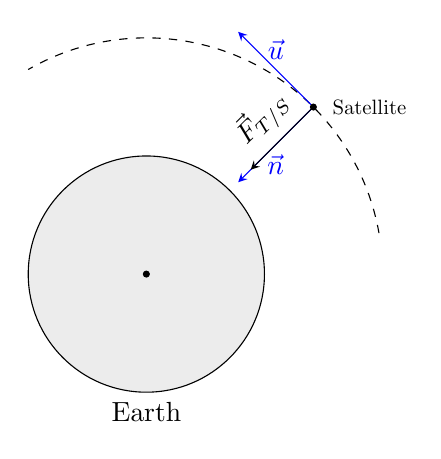
\begin{tikzpicture}[>=stealth, scale=1.5]
%The circle represents the earth and I filled it with gray
\draw[fill=lightgray!30!white] (0,0)circle(1);
%this dot represents the earth's center of gravity
\filldraw[black] (0,0)circle(0.025) node[below=1.5] {Earth};
%the satellite's path
\draw[dashed] (10:2)arc[start angle=10,end angle=120,x radius=2cm,y radius=2cm];
%The gravitational force + frenet base 
\begin{scope}[shift={(45:2)}, rotate=45]
\draw[->, blue] (0,0)--(0,0.9)node[midway, above] {$\vec{u}$};
\draw[->, blue] (0,0)--(-0.9,0) node[below, midway] {$\vec{n}$};
\draw[->] (0,0)--(-0.75,0) node[midway, above, rotate=45] {$\vec{F}_{T/S}$};
%This dot represents the satellite
\filldraw[black] (0,0)circle(0.025) node[right=0.15, scale=0.75] {Satellite};
\end{scope}
\end{tikzpicture}
\end{document}
